% Results

\subsection*{PSSM}

C programs from the course were used to estimate MHC binding affinity with PSSM. 
Here a threshold must be used to limit included peptides to the ones that actually bind to the MHC molecule. 
In the machine learning methods non-binding data is also be valuable in the estimation.

All entries from the training data set with binding affinity over 0.426 are feeded into a program. 
This value means that the peptide successfully binds to the MHC molecule. All peptides should be of same length.
The Blosum frequency substitution matrix, is a
conditional probability matrix of matching amino
acids j given you have amino acid i

\begin{equation}
P(j|i) = \frac{P_ij}{Q_i}
\end{equation}

The matrix is used to. The result is a PSSM matrix. 

Experimental data from the HLA-A*0201 allele is randomly split up in training and evaluation sections, the evaluation section being 1/5 of the training data size (618 peptides vs 2471 peptides in the training set).
For 5 different samplings we get a Pearson correlation coefficients of {0.75323,, 0.78415, 0.78009, 0.78896, 0.76480}, the average being 0.774.
The corresponding results without using sequence weighting are {0.73530, 0.75961, 0.75791, 0.76343, 0.74639}, with average of 0.753
Using identity matrix instead of the blosum substitiution matrix gives similar values {0.75107, 0.77989, 0.74344, 0.78552, 0.76072} with average of 0.764.
The blosum matrix is not making a difference here as substitution frequencies should not affect much binding affinity of a peptide in a MHC molecule.

We also try the smaller set HLA-A3001. It has a total of 669 experimentally verified peptides.
Using the blosum matrix the correlation results are {0.69872, 0.55787, 0.65032, 0.55827, 0.57044}, an average of 0.607
The corresponding results without using sequence weighting are {0.67775, 0.54853, 0.63731, 0.55026, 0.56416}, with average of 0.596
The identity matrix gives results of with average of (0.63987 0.45267 0.55898 0.49296 0.49224) 0.527 

Using a small dataset the benefit of using a blosum frequency substitution matrix is greater.

\begin{table}[ht]
\begin{center}
\begin{tabular}{rllrrr}
  \hline
 & Param & Allele & Sample & Size & PCC \\ 
  \hline
 & PSSM w/o SW & A0201 &   0 & 618 & 0.74 \\ 
 & PSSM w/o SW & A0201 &   1 & 618 & 0.76 \\ 
 & PSSM w/o SW & A0201 &   2 & 618 & 0.76 \\ 
 & PSSM w/o SW & A0201 &   3 & 618 & 0.76 \\ 
 & PSSM w/o SW & A0201 &   4 & 617 & 0.75 \\ 
\hline
 & PSSM w SW & A0201 &   0 & 618 & 0.75 \\ 
 & PSSM w SW & A0201 &   1 & 618 & 0.78 \\ 
 & PSSM w SW & A0201 &   2 & 618 & 0.78 \\ 
 & PSSM w SW & A0201 &   3 & 618 & 0.79 \\ 
 & PSSM w SW & A0201 &   4 & 617 & 0.76 \\ 
   \hline
\end{tabular}
\end{center}
\label{tab:pssm1}
\caption{PSSM table A0201}
\end{table}

\begin{table}[ht]
\begin{center}
\begin{tabular}{rllrrr}
  \hline
 & Param & Allele & Sample & Size & PCC \\ 
  \hline
   & PSSM & A3001 &   0 & 134 & 0.68 \\ 
   & PSSM & A3001 &   1 & 134 & 0.55 \\ 
   & PSSM & A3001 &   2 & 134 & 0.64 \\ 
   & PSSM & A3001 &   3 & 134 & 0.55 \\ 
   & PSSM & A3001 &   4 & 133 & 0.56 \\ 
  \hline
   & PSSM SW & A3001 &   0 & 134 & 0.70 \\ 
   & PSSM SW & A3001 &   1 & 134 & 0.56 \\ 
   & PSSM SW & A3001 &   2 & 134 & 0.65 \\ 
   & PSSM SW & A3001 &   3 & 134 & 0.56 \\ 
   & PSSM SW & A3001 &   4 & 133 & 0.57 \\ 
   \hline
\end{tabular}
\end{center}
\label{tab:pssm2}
\caption{PSSM table A3001}
\end{table}

\begin{figure*}
\begin{center}
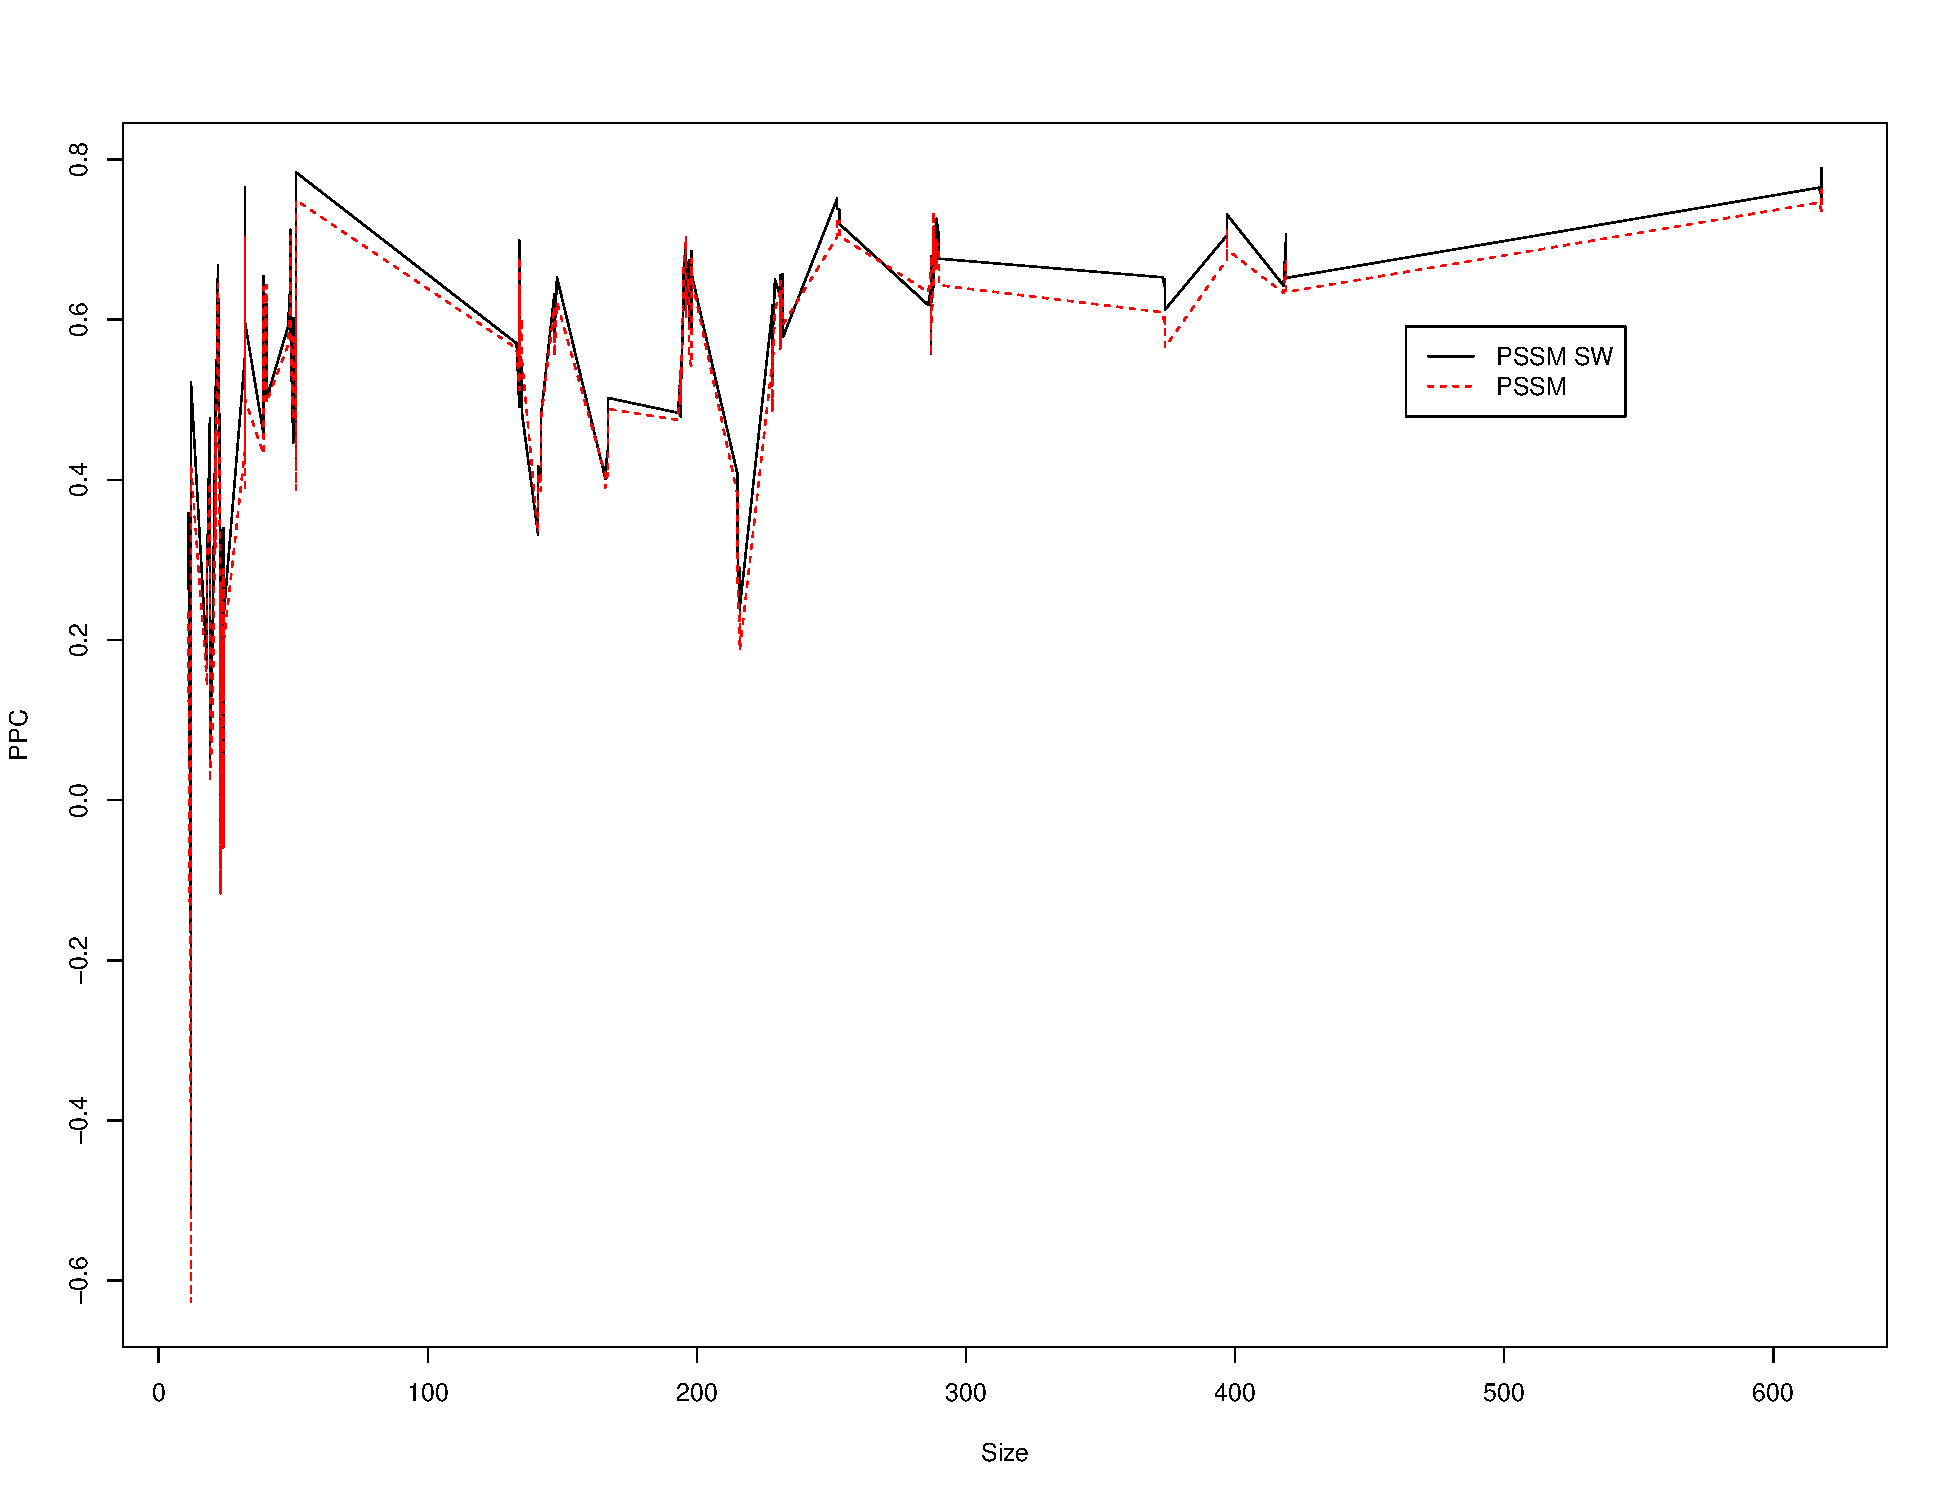
\includegraphics[width=12cm]{fig/pssm1.pdf}
\label{fig:pssm1}
\caption{PSSM Results}
\end{center}
\end{figure*}

\subsection*{SVM}
There exists a fairly well established programming library for SVM calculations, libsvm, but in this investigation version 3.6.3 of the java based Weka sofware is used. 
The data has to be prepared for input into the Weka program.
The number of amino acids is 20 and the length of the peptide is 9 so each peptide is changed to a vector of length 20*9. 
Three encoding schemes are used, blostum50, sparse and z-score. 
In the case of the blosum encoding scheme, each of the 9 sections of length 20 simply contain the data from each row in blosum matrix corresponding to the amino acid in question.
The sparse encoding simply uses the identity substitution matrix similar to the one in the PSSM case. 
The z-score encoding is a condensed manner to represent each amino acid, only 5 values are used to encode each amino acid based on on their properties. 
These properties were deduced from measured data using thin-layer chromatography and nuclear magnetic resonance and some calculated variables 
such as side chain charge, hydrogren bond donor and acceptor properties, log P and molecular weight. 
Each row in the input matrix has therefore length of 5*20+1 (the one being the measured affinity value)
The same data as from the PSSM section is used for comparison. For the HLA-A*0201 dataset and sparse encoding we get the results displayed in table \ref{tab:svm1}.

\begin{table}[ht]
\begin{center}
\begin{tabular}{ ll c r }
\hline
 & Correlation coefficient &                 0.78  \\
 & Mean absolute error      &                0.1524 \\
 & Root mean squared error   &               0.1925 \\
 & Relative absolute error    &             57.0908\%  \\
 & Root relative squared error &            62.8014\%  \\
 & Total Number of Instances    &          618 \\
\hline
\end{tabular}
\label{tab:svm1}
\caption{SVM Results 1}
\end{center}
\end{table}


The SMOreg classifier (Table \ref{tab:svm2}) with polynomial kernel of first degree we give just slightly better results than the PSSM. Rising the degree of the kernel to 2 does not give better results.

\begin{table}[ht]
\begin{center}
\begin{tabular}{ ll c r }
\hline
 & Correlation coefficient &                 0.756 \\
 & Mean absolute error      &                0.1535 \\
 & Root mean squared error   &               0.2039 \\
 & Relative absolute error   &              57.5209\% \\
 & Root relative squared error &            66.4967\% \\
 & Total Number of Instances    &          618 \\
\hline
\end{tabular}
\label{tab:svm2}
\caption{SVM Results 2}

\end{center}
\end{table}

Using the blosum matrix with kernel degree of 1 we have the results displayed in Table \ref{tab:svm3}. Polynomial kernel of degree 2 has considerably worse performance for the blosum encoded data (see Tab \ref{tab:svm4}). Also the z-score encoded data with polynomial kernel of degree 1 (Tab \ref{tab:svm5}) haven't better results.



\begin{table}[ht]
\begin{center}
\begin{tabular}{ ll c r }
\hline
 & Correlation coefficient  &                0.7789 \\
 & Mean absolute error       &               0.1533 \\
 & Root mean squared error   &               0.1928 \\
 & Relative absolute error   &              57.4187\% \\
 & Root relative squared error  &           62.8817\% \\
 & Total Number of Instances     &         618  \\
\hline
\end{tabular}
\label{tab:svm3}
\caption{SVM Results 3}
\end{center}
\end{table}

\begin{table}[ht]
\begin{center}
\begin{tabular}{ ll c r }
\hline
 & Correlation coefficient                  0.6692 \\
 & Mean absolute error                      0.2047 \\
 & Root mean squared error                  0.262 \\
 & Relative absolute error                 76.6914\% \\
 & Root relative squared error             85.4726\% \\
 & Total Number of Instances              618  \\
\hline
\end{tabular}
\label{tab:svm4}
\caption{SVM Results 4}
\end{center}
\end{table}


\begin{table}[ht]
\begin{center}
\begin{tabular}{ ll c r }
\hline
 & Correlation coefficient   &              0.6888 \\
 & Mean absolute error        &              0.1802 \\
 & Root mean squared error    &              0.2227 \\
 & Relative absolute error    &             67.5222\% \\
 & Root relative squared error &             72.6292\% \\
 & Total Number of Instances   &           618     \\
\hline
\end{tabular}
\label{tab:svm5}
\caption{SVM Results 5}
\end{center}
\end{table}

Trying the same tests in a smaller dataset, the HLA-A*3001 (Tab \ref{tab:svm6}), we nitice that a polynomial kernel of degree 2 slightly rises the prediction performance (Tab \ref{tab:svm7}).

\begin{table}[ht]
\begin{center}
\begin{tabular}{ ll c r }
\hline
 & Correlation coefficient       &           0.7412 \\
 & Mean absolute error            &          0.1008 \\
 & Root mean squared error        &          0.1473 \\
 & Relative absolute error        &         70.3882\% \\
 & Root relative squared error    &         68.5173\% \\
 & Total Number of Instances      &        134 \\
\hline
\end{tabular}
\label{tab:svm6}
\caption{SVM Results 6}
\end{center}
\end{table}


\begin{table}[ht]
\begin{center}
\begin{tabular}{ ll c r }
\hline
 & Correlation coefficient        &          0.7671 \\
 & Mean absolute error            &          0.0945 \\
 & Root mean squared error        &          0.1424 \\
 & Relative absolute error        &         65.9762\% \\
 & Root relative squared error    &         66.2741\% \\
 & Total Number of Instances      &        134 \\
\hline
\end{tabular}
\label{tab:svm7}
\caption{SVM Results 7}
\end{center}
\end{table}

\subsection*{ANN}

\begin{figure*}
\begin{center}
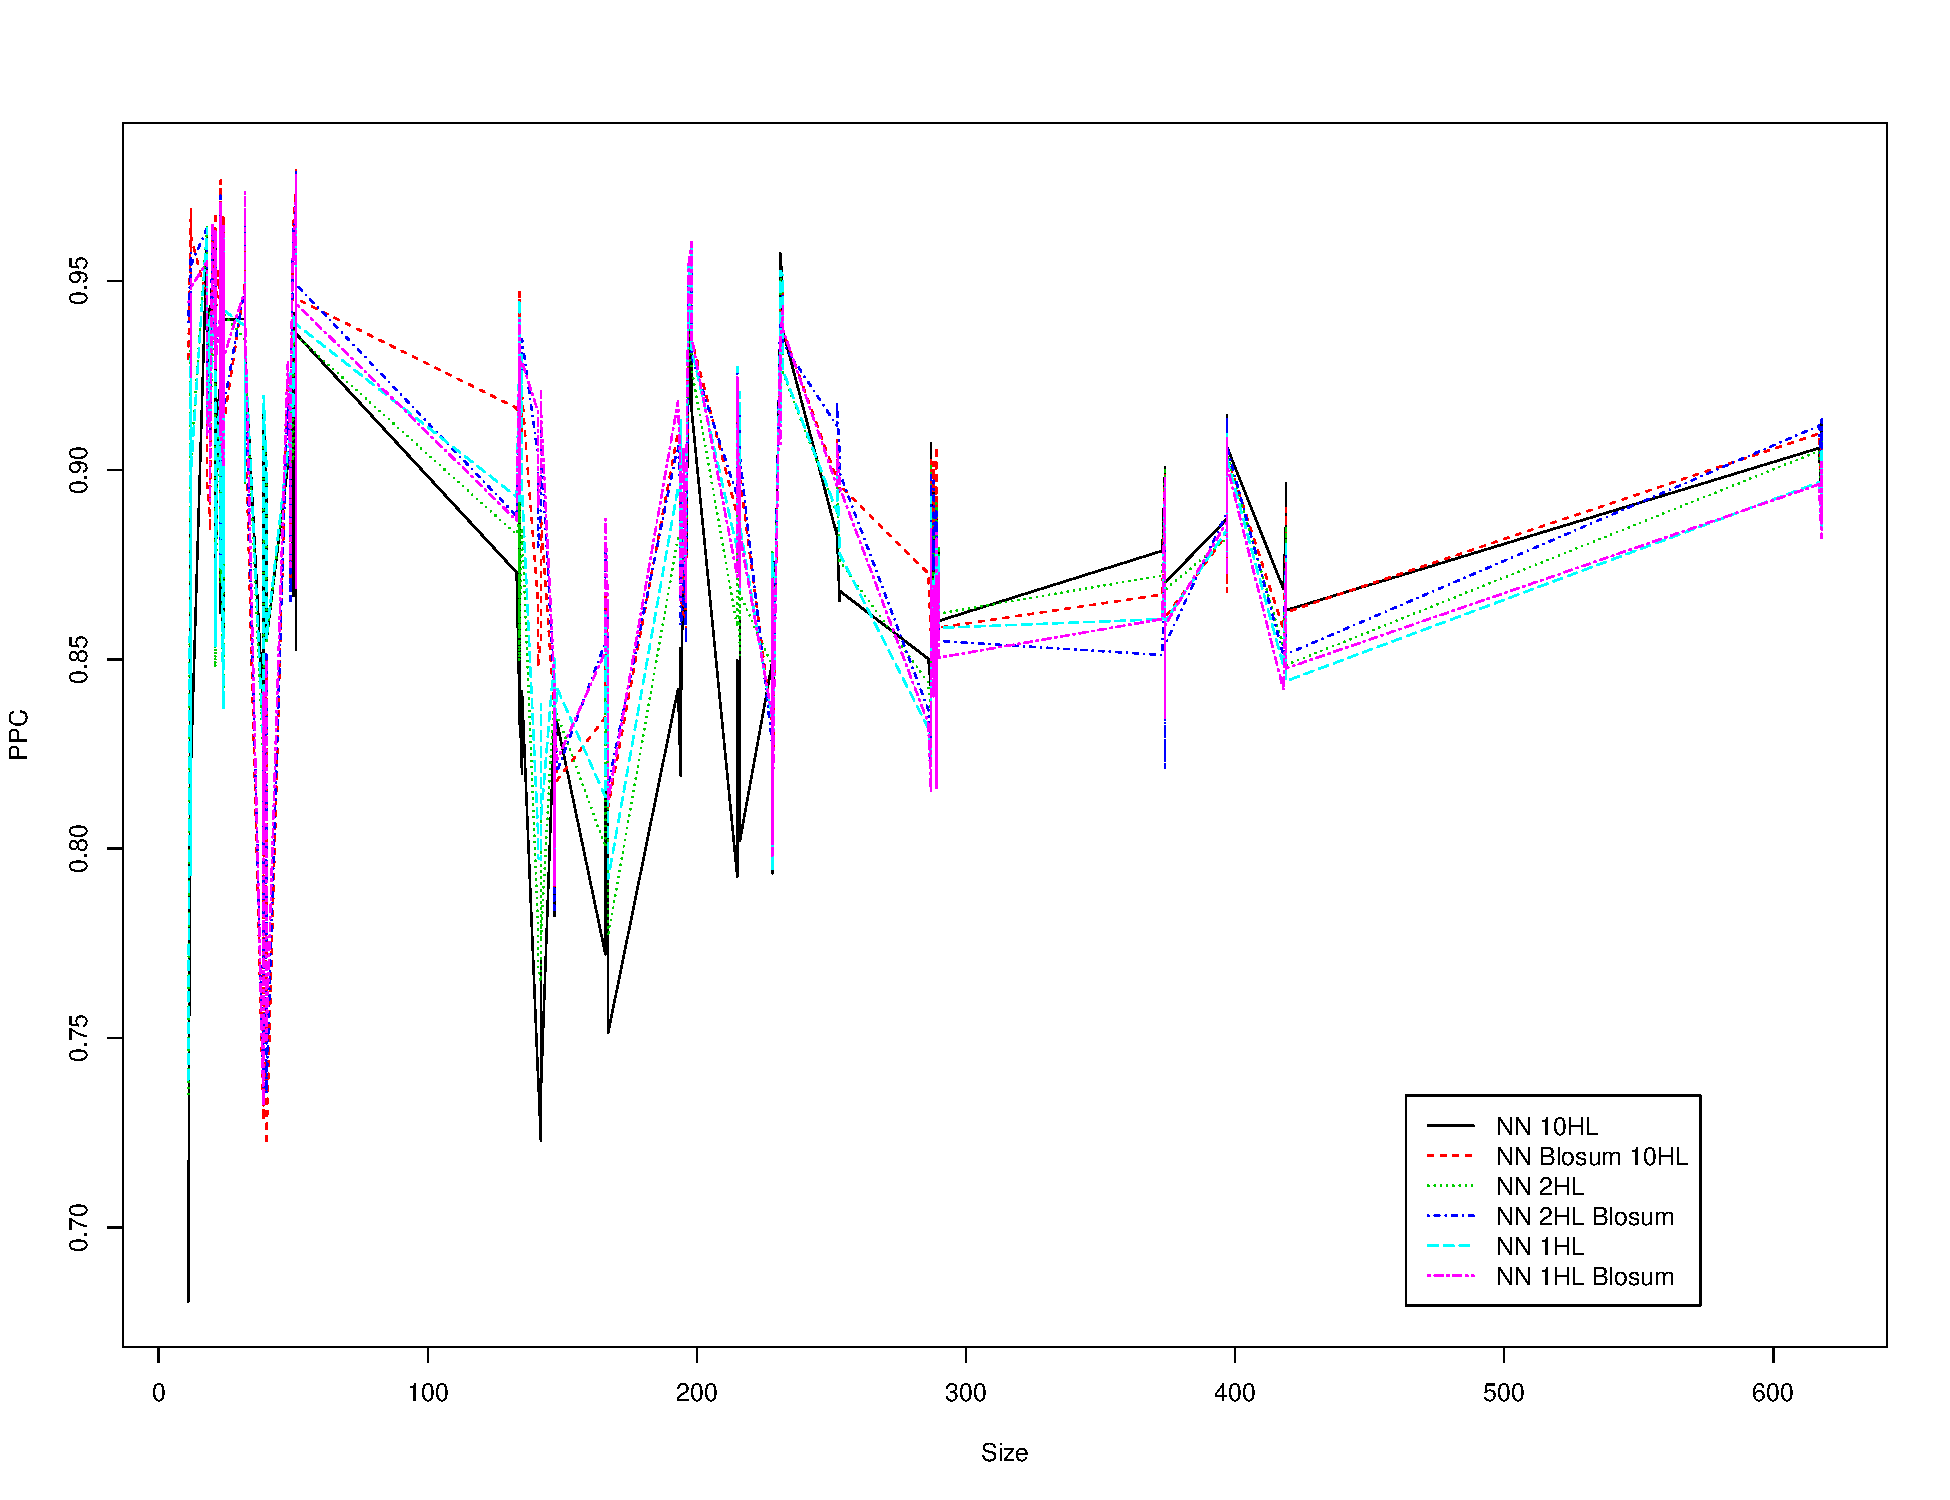
\includegraphics[width=12cm]{fig/ann1.pdf}
\label{fig:ann1}
\caption{Artificial Neuronal Network Results}
\end{center}
\end{figure*}

\begin{table}[ht]
\begin{center}
\begin{tabular}{rllrrr}
  \hline
 & Param & Allele & Sample & Size & PCC \\ 
  \hline
 & NN 10HL & A0201 &   0 & 618 & 0.89 \\ 
   & NN 10HL & A0201 &   1 & 618 & 0.91 \\ 
   & NN 10HL & A0201 &   2 & 618 & 0.90 \\ 
   & NN 10HL & A0201 &   3 & 618 & 0.90 \\ 
   & NN 10HL & A0201 &   4 & 617 & 0.91 \\ 
   \hline
   & NN Blosum 10HL & A0201 &   0 & 618 & 0.89 \\ 
   & NN Blosum 10HL & A0201 &   1 & 618 & 0.91 \\ 
   & NN Blosum 10HL & A0201 &   2 & 618 & 0.90 \\ 
   & NN Blosum 10HL & A0201 &   3 & 618 & 0.91 \\ 
   & NN Blosum 10HL & A0201 &   4 & 617 & 0.91 \\ 
   \hline
   & NN 1HL & A0201 &   0 & 618 & 0.89 \\ 
   & NN 1HL & A0201 &   1 & 618 & 0.91 \\ 
   & NN 1HL & A0201 &   2 & 618 & 0.89 \\ 
   & NN 1HL & A0201 &   3 & 618 & 0.89 \\ 
   & NN 1HL & A0201 &   4 & 617 & 0.90 \\ 
   \hline
   & NN 1HL Blosum & A0201 &   0 & 618 & 0.88 \\ 
   & NN 1HL Blosum & A0201 &   1 & 618 & 0.90 \\ 
   & NN 1HL Blosum & A0201 &   2 & 618 & 0.89 \\ 
   & NN 1HL Blosum & A0201 &   3 & 618 & 0.89 \\ 
   & NN 1HL Blosum & A0201 &   4 & 617 & 0.90 \\ 
   \hline
   & NN 2HL & A0201 &   0 & 618 & 0.89 \\ 
   & NN 2HL & A0201 &   1 & 618 & 0.91 \\ 
   & NN 2HL & A0201 &   2 & 618 & 0.90 \\ 
   & NN 2HL & A0201 &   3 & 618 & 0.90 \\ 
   & NN 2HL & A0201 &   4 & 617 & 0.91 \\ 
   \hline
   & NN 2HL Blosum & A0201 &   0 & 618 & 0.90 \\ 
   & NN 2HL Blosum & A0201 &   1 & 618 & 0.91 \\ 
   & NN 2HL Blosum & A0201 &   2 & 618 & 0.90 \\ 
   & NN 2HL Blosum & A0201 &   3 & 618 & 0.91 \\ 
   & NN 2HL Blosum & A0201 &   4 & 617 & 0.91 \\ 
   \hline
\end{tabular}
\label{tab:nn1}
\caption{Artificial Neuronal Network for A0201}
\end{center}
\end{table}



